% LaTeX file for Chapter 01



%  possible title: Causal inference for non-randomized data and heterogeneous treatment effect estimation


\chapter{Introduction}

\section{Motivation}

% Why, what and how\dots

The most important questions in research are mostly not associational, but causal \citep{pearl2009}. They concern the effects of interventions -- such as the impact of a treatment -- or seek explanations for observed outcomes, such as identifying which disease caused certain symptoms. They also include hypothetical scenarios; for example: what would the GDP have been if interest rates had increased by 25 instead of 75 basis points? Answering such questions requires causal reasoning and demands an understanding of the underlying data-generating process. Purely associational approaches are typically not sufficient to draw valid causal conclusions.

% https://ascpt.onlinelibrary.wiley.com/doi/epdf/10.1002/cpt.3159
% One of the main reasons for this is thatML methods are particularly good at learning about the status quofrom existing data to ultimately make outcome predictions thatare exactly in line with the current distribution of data character-istics, but usually not designed for tasks that involve the need toreason about interventions on the data generating distributionsleading to counterfactual scenarios,


The gold standard for estimating the causal effect of an intervention on an outcome is the randomized controlled trial (RCT) \citep{hariton2018}. In this prospective study design, participants are randomly assigned to either the treatment or control group. Randomization aims to eliminate the influence of potential confounding variables, ensuring that treatment groups are balanced with respect to baseline characteristics. This allows for an unbiased estimation of the causal effect. Despite their strengths, RCTs have several limitations. They are often expensive and time-consuming to plan and execute. Moreover, the results may not generalize well to the population of interest, as individuals who volunteer or are accepted for trials are not always representative of the target group. Additionally, RCTs typically estimate an average treatment effect (ATE) on a sample, which is the difference in mean outcomes between treatment arms \citep{nichols2007}. However, individual patients may respond differently to the treatment, depending on their unique characteristics. In the context of personalized medicine, it is therefore crucial to have an estimate of treatment effects at the individual level. Another central limitation of RCTs is that in many scenarios they can simply not be conducted due to ethical or practical reasons. For example, an RCT is only ethical in the case of clinical equipoise, which means that there is uncertainty about the (superiority) of one of the two treatment arms \citep{freedman1987}. It is not acceptable to treat one group with the assumed inferior treatment. The same is true for obviously harmful interventions, like smoking or drinking alcohol. In these cases, it is not possible to conduct an RCT to estimate the causal effect of smoking on lung cancer. 

For these reasons, much of research aims to make causal inference from observational data, using non-experimental or quasi-experimental designs. Unlike RCTs, these settings do not involve randomization to treatment, which introduces challenges due to confounding. Methods for causal inference from observational data aim to correctly control for such confounders to enable valid causal conclusions. Recently, \citet{sick2025} proposed the TRAM-DAGs framework, which estimates the functional form of causal relationships in a known causal graph based on observational or RCT data and make subsequent causal queries. In this thesis we further analyze and apply this method.

As mentioned earlier, an application where causal inference is of particular importance is the estimation of personalized treatment effects. In personalized medicine, this is referred to as the individualized treatment effect (ITE) or conditional average treatment effect (CATE), while in business and marketing contexts, the term uplift modeling is often used (\citealp{gutierrez2017}; \citealp{zhao2020}). These concepts refer to the difference in potential outcomes under different treatments, assessed at the level of individuals or subgroups. Such estimates are critical in settings where treatment responses vary significantly between individuals. For clinical decision-making, tailoring therapies to individual characteristics can lead to more effective and efficient care. The importance of estimating individual-level effects is not limited to medicine. It also is of high interest in marketing, where campaigns can be precisely targeted to maximize impact and minimize adverse responses. Consider, for instance, the decision of whether to send a push notification (treatment) to a customer. Some customers might be persuadables, who will respond positively only if treated. Others, in contrast, might have responded positively without the intervention but are negatively affected by it -- for example, a customer who is reminded of a forgotten subscription and, as a result, decides to cancel it. In this context, identifying persuadables is valuable, while treating the latter may be counterproductive. This illustrates the need to understand treatment effects at a granular level to guide individualized decisions.
Various methods have been proposed to estimate individualized treatment effects, yet this task remains challenging. The fundamental problem is that only one of the two potential outcomes can ever be observed for any given individual, making the estimation of treatment effects inherently more difficult than standard predictive modeling.

% \citep{gutierrez2017, zhao2020}








\section{Key concepts of causal inference}

Causal relationships can be represented by a directed acyclic graph (DAG), as shown in Figure \ref{fig:pearl_levels}(a). The variables, or nodes, are connected by directed edges, which represent causal dependencies.

% Visual examples of these levels are presented in Figure~\ref{fig:pearl_levels}(a)--(c). redundant, later i refer to it again
Questions in causal inference are typically classified into one of the three levels of Pearl's hierarchy of causation \citep{pearl_book2009}. Level 1 corresponds to observational queries, expressed as conditional probabilities $P(Y \mid X)$, which can be answered directly from the joint distribution $P(Y \cap X)$. Level 2 involves interventional queries, such as $P(Y \mid do(X))$, which describe the probability when actively setting a variable $X$ to a particular value. Unlike observational queries, answering interventional questions requires knowledge of the underlying causal structure. Level 3 addresses counterfactual reasoning, which poses the greatest challenge. These are hypothetical what-if questions that require reasoning about outcomes under alternative realities. For example, if a patient received a treatment and died, the factual outcome is death under the received treatment. The counterfactual would be the outcome that would have occurred had the patient received a different treatment.

 
Some statisticians argue that counterfactuals -- being unobservable and untestable -- are of limited scientific value and may be regarded as metaphysical \citep{dawid2000}. Nevertheless, there are important practical questions that require the analysis of such counterfactuals.



% include image /img/pearl_levels.png
\begin{figure}[H]
\centering
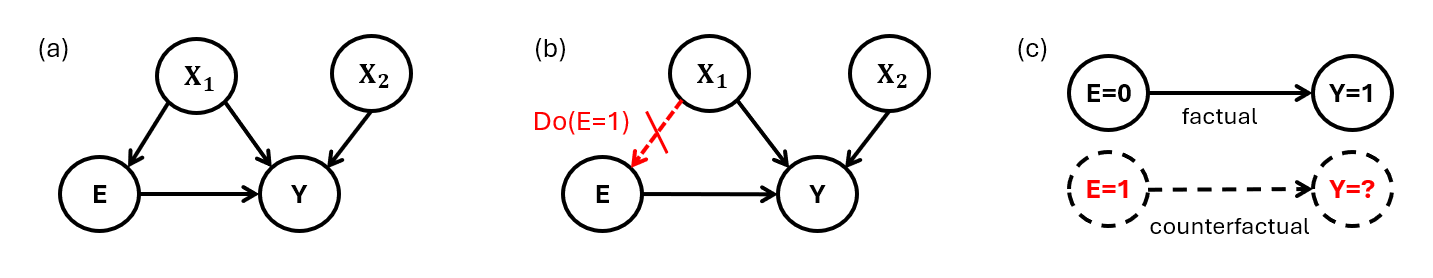
\includegraphics[width=1\textwidth]{img/pearl_levels.png}
\caption{Example for the three levels of Pearl's hierarchy of causation. (a) DAG for observational data. (b) DAG when making a do-intervention by fixing the variable E at a certain value. c) Observed factual outcome and corresponding counterfactual query.}
\label{fig:pearl_levels}
\end{figure}


To illustrate Pearl's three levels of causality, I consider a simplified example involving the exposure Exercise ($E$), the outcome Heart Disease ($Y$), the confounder Age ($X_1$) and the additional covariate Smoking ($X_2$). I assume that exercise reduces the risk of heart disease, but both variables are also influenced by age. Figure \ref{fig:pearl_levels}(a)--(c) illustrates the corresponding scenarios.





\textbf{Level 1: Observational ("seeing"):}  
We observe the joint distribution of variables without intervention.  
Example: What is the probability of heart disease given that a person exercises?  
\[
P(Y = 1 \mid E = 1)
\]
This can be estimated directly from data by conditioning on $E = 1$ and computing the frequency of $Y$. However, such an estimate does not account for confounding variables like age.



\textbf{Level 2: Interventional ("doing"):}  
We consider the effect of actively intervening in the system.  
Example: What is the probability of heart disease if everyone were made to exercise, regardless of age or smoking status?  
\[
P(Y = 1 \mid \text{do}(E = 1))
\]
Answering this requires assumptions about the underlying causal structure.



\textbf{Level 3: Counterfactual ("imagining"):}  
We ask what would have happened under different circumstances -- that is, we imagine an alternative scenario for the same individual.  
Example: For a person who does not exercise and has heart disease, would they still have had heart disease if they had exercised?  
\[
P(Y_{E=1} \mid E = 0, Y = 1)
\]
Here, $Y_{E=1}$ represents the counterfactual outcome under positive exposure. Counterfactual queries require a structural causal model (SCM) and cannot be answered from data alone. 

Here, $Y_{E=1}$ represents the counterfactual outcome under positive exposure. Counterfactual queries cannot be answered from observational data alone; they require a structural framework that explicitly models the data-generating process. 


% With our new framework, we can answer all three types of questions, with a small exception for Counterfactuals in the non-continuous case.



% the following all from pearl book p. 27
For this, the concept of DAGs can be extended to structural causal model (SCM). A set of structural equations of the form $X_i = f_i(\text{pa}(X_i), Z_i), \quad i = 1, \dots, n$ build a structural causal model \citep{pearl_book2009}.  $\text{pa}(X_i)$ denotes the direct causal parents of $X_i$, and $Z_i$ is an exogenous noise variable. These exogenous variables capture latent factors that influence $X_i$ but are not explicitly modeled. By convention, the $Z_i$ are assumed to be mutually independent.

Each function $f_i$ -- which may be nonlinear -- defines how the value of $X_i$ is generated from its parents and the corresponding noise term. A source node $X_j$ without any parents is modeled as $X_j = f_j(Z_j)$. Once all structural equations and noise variables are specified, the model is fully deterministic in the sense that each variable is a fixed function of its parents and its own exogenous noise. The randomness in the system arises entirely from these independent noise terms, which encode unobserved factors. This functional representation makes it possible to compute interventional distributions and evaluate counterfactual outcomes. These aspects are discussed in detail in Section~\ref{methods:sampling}.


In this thesis, we do not focus on discovering the underlying causal graph. Such a structure may be obtained through structure learning algorithms or determined from expert knowledge. Instead, we assume the graph is known and concentrate on estimating the functional form of the relationships between variables -- that is, the structural equations that define the SCM.

Various approaches exist for estimating the functions $f_i$ that constitute an SCM, depending on the assumptions made about the data and the model class. These methods are discussed in the next section.




% \[
% X_i = \beta_0 + \beta_1 X_{pa(x_i)} + Z_i
% \]
%
% \[
%   X \sim \mathcal{N}(\mu = pa(X)\beta,\,\sigma^{2})\,.
% \]


A simple approach to modeling the structural equations is linear regression, which assumes Gaussian error terms $Z_i$ and linear functional forms $f_i$. Classical statistical methods of this kind are typically well-defined, computationally efficient, and offer interpretable parameters. However, they rely on strong assumptions about the underlying data-generating mechanism -- such as linearity and homoscedasticity -- which may not hold in practice. Violations of these assumptions can lead to biased or misleading results.

Alternatively, more flexible approaches based on neural networks have gained popularity for estimating structural equations. These models are capable of approximating complex, nonlinear relationships and capturing complicated interactions between variables with minimal bias. Their flexibility, however, often comes at the cost of reduced interpretability and, in some cases, limited applicability to non-continuous or mixed data types. \citet{poinsot2024} provided an overview of deep structural causal models and their use in counterfactual inference.

The TRAM-DAG framework proposed by \citet{sick2025} builds a bridge between these classical and neural-network-based modeling approaches, by combining interpretable transformation models with the flexibility of neural networks. At its core, the structural equations are modeled using transformation models \citep{hothorn2014}, a flexible class of distributional regression methods. These models were subsequently extended to deep transformation models (Deep TRAMs) by \citet{sick2020}, enabling the use of neural networks to parameterize conditional distributions in a customizable way. In the TRAM-DAG framework, these deep TRAMs are applied according to a known causal graph, allowing the model to be fitted to observational data and used to answer causal queries across all three levels of Pearl's hierarchy. The framework is introduced in more detail in Section~\ref{sec:tram_dags}.





\section{Goals and contributions} \label{sec:goals_contributions}

This thesis contributes to the further exploration of the TRAM-DAG framework and to adressing challenges in the estimation of personalized treatment effects.

The first part of this thesis focuses on a systematic analysis and extension of TRAM-DAGs. This includes applying the model across a variety of settings, such as different data types, model complexities, and neural network configurations (e.g., activation functions, batch normalization, dropout). Most analyses are conducted on simulated data to know the underlying data-generating process, but the model is also applied to real-world data to demonstrate its practical utility.

The second focus of the thesis is on the estimation of personalized treatment effects. Recent work by \citet{chen2025} showed that most causal machine learning models trained on RCT data failed to generalize when evaluated out of sample. In this thesis, we replicate some of their work by applying various models, including TRAM-DAGs, to the same data and analyzing whether we come to a similar conclusion. We further investigate why individualized treatment effect (ITE) estimation can fail in such settings, and under which conditions reliable estimates can be obtained. In addition, we demonstrate that TRAM-DAGs can be effectively used to estimate ITEs even in non-randomized observational settings, provided that the causal graph is known and fully observed. In doing so, we explore the potential of TRAM-DAGs as a framework for answering complex causal questions across different levels of Pearl's hierarchy.



Formally, we aim to answer following research questions in this thesis:

\begin{itemize}
    \item How can TRAM-DAGs be applied under different scenarios such as ordinal predictors, scaled vs. raw variables or allowing for interactions between variables.
    \item Do we obtain similar results when estimating ITEs on a real-world RCT dataset, as reported by \citet{chen2025}?
    \item What are possible reasons for the failure of ITE estimation in some cases when causal machine learning models are validated out of sample?
    \item How can TRAM-DAGs be used to estimate ITEs in both randomized controlled trials and observational settings involving confounding and mediating variables?
\end{itemize}



With this work, we aim to contribute to the important and evolving field of causal inference in observational settings and to the challenging task of estimating individualized treatment effects.
